\exercisesheader{}

% 31 - pickup

\eoce{\qt{Used trucks\label{pickup}} The scatterplot below shows the relationship between year and price (in thousands of \$) of a random sample of 42 pickup trucks. Also shown is a residuals plot for the linear model for predicting price from year.
\begin{center}
\tabspecial{tableau-usedtrucks}{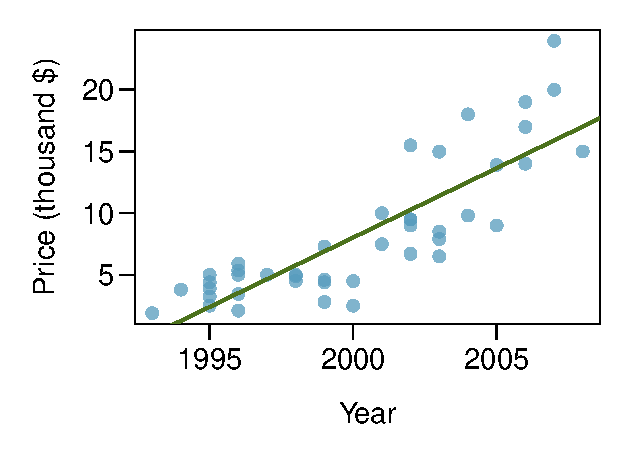
\includegraphics[width=0.42\textwidth]{ch_regr_simple_linear/figures/eoce/pickup/pu_lin_scat}} 
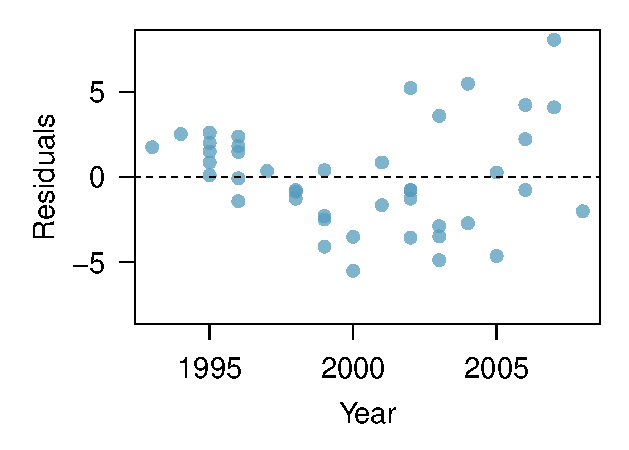
\includegraphics[width=0.42\textwidth]{ch_regr_simple_linear/figures/eoce/pickup/pu_res_scat}
\end{center}
\begin{parts}
\item Describe the relationship between these two variables and comment on whether a linear model is appropriate for modeling the relationship between year and price.
\item The scatterplot below shows the relationship between logged (natural log) price and year of these trucks, as well as the residuals plot for modeling these data. Comment on which model (linear model from earlier or logged model presented here) is a better fit for these data.
 \begin{center}
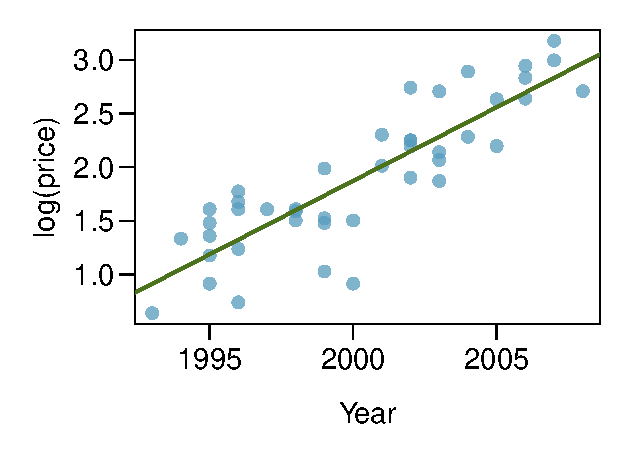
\includegraphics[width=0.42\textwidth]{ch_regr_simple_linear/figures/eoce/pickup/pu_lin_scat_log} 
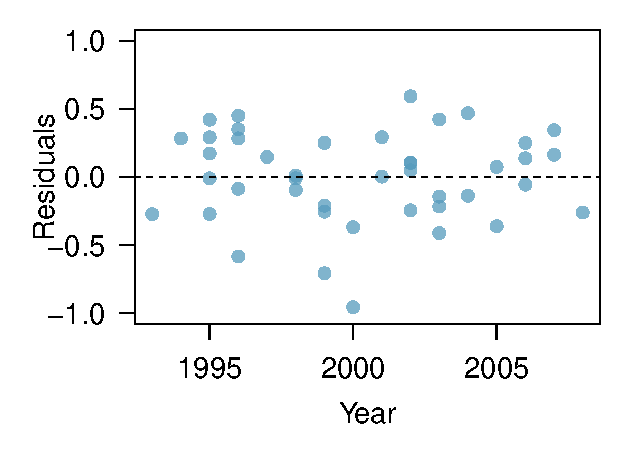
\includegraphics[width=0.42\textwidth]{ch_regr_simple_linear/figures/eoce/pickup/pu_res_scat_log} 
\end{center}
\item The output for the logged model is given below. Interpret the slope in context of the data.
\begin{center}
\begin{tabular}{rrrrr}
  \hline
 & Estimate & Std. Error & t value & Pr($>$$|$t$|$) \\ 
  \hline
(Intercept) & -271.981 & 25.042 & -10.861 & 0.000 \\ 
Year & 0.137 & 0.013 & 10.937 & 0.000 \\ 
   \hline
\end{tabular}
\end{center}
\end{parts} 
}{}

\D{\newpage}
% 32 - income_hours_worked_ap

\eoce{\qt{Income and hours worked\label{income_hours_worked_ap}} The scatterplot below shows the relationship between income and years worked for a random sample of 787 Americans. Also shown is a residuals plot for the linear model for predicting income from hours worked. The data come from the 2012 American Community Survey.\footfullcite{data:acs:2012} 
\begin{center}
\tabspecial{tableau_income_hours_worked}{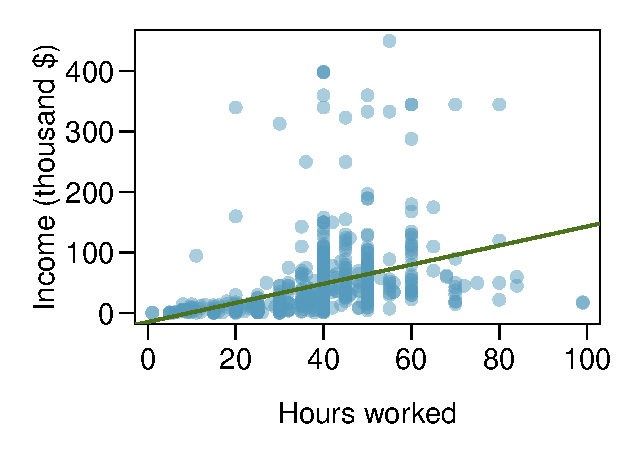
\includegraphics[width=0.42\textwidth]{ch_regr_simple_linear/figures/eoce/income_hours_worked_ap/acs_lin_scat} }
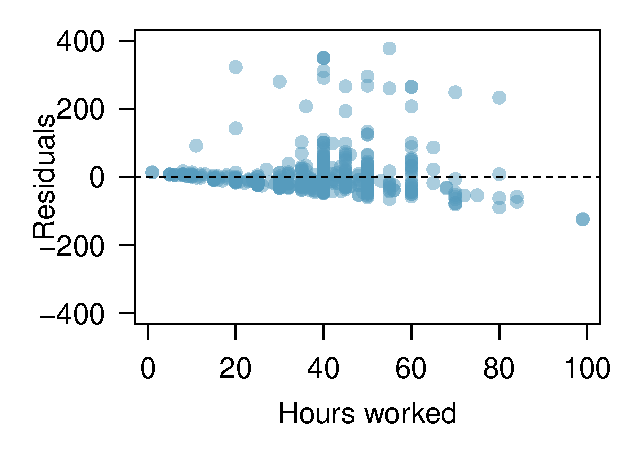
\includegraphics[width=0.42\textwidth]{ch_regr_simple_linear/figures/eoce/income_hours_worked_ap/acs_lin_res_scat} 
\end{center}
\begin{parts}
\item Describe the relationship between these two variables and comment on whether a linear model is appropriate for modeling the relationship between year and price.
\item The scatterplot below shows the relationship between logged (natural log) income and hours worked, as well as the residuals plot for modeling these data. Comment on which model (linear model from earlier or logged model presented here) is a better fit for these data.
 \begin{center}
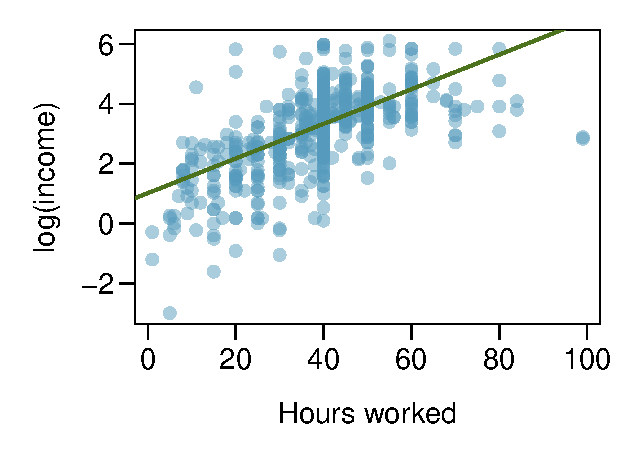
\includegraphics[width=0.42\textwidth]{ch_regr_simple_linear/figures/eoce/income_hours_worked_ap/acs_log_scat.pdf} 
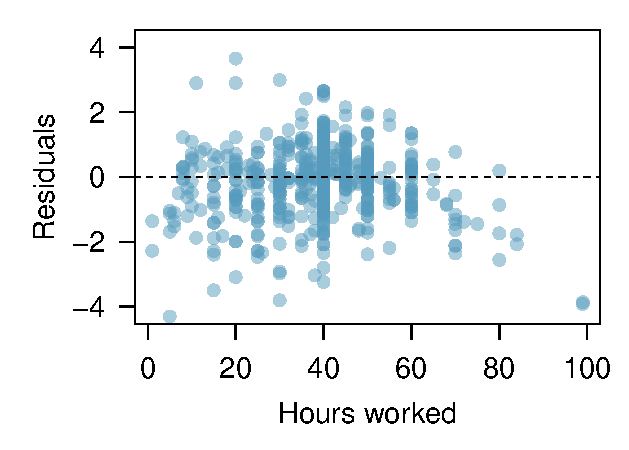
\includegraphics[width=0.42\textwidth]{ch_regr_simple_linear/figures/eoce/income_hours_worked_ap/acs_log_res_scat.pdf} 
\end{center}
\item The output for the logged model is given below. Interpret the slope in context of the data.
\begin{center}
\begin{tabular}{rrrrr}
  \hline
 & Estimate & Std. Error & t value & Pr($>$$|$t$|$) \\ 
  \hline
(Intercept) & 1.017 & 0.113 & 9.000 & 0.000 \\ 
  hrs\_work & 0.058 & 0.003 & 21.086 & 0.000 \\ 
   \hline
\end{tabular}
\end{center}
\end{parts} 
}{}
